\documentclass{article}
\usepackage[margin=2.2cm]{geometry}
\usepackage{booktabs}
\usepackage{array}
\usepackage{longtable}
\usepackage{float}
\usepackage[table]{xcolor}
\usepackage{hyperref}
\usepackage[utf8]{inputenc}
\usepackage{tikz}
\newcommand{\INF}{$\infty$}
\title{Proyecto 1 – Floyd–Warshall}
\author{Fabian Bustos - Esteban Secaida}
\date{\today}
\begin{document}
\maketitle
\section*{Grafo de rutas}
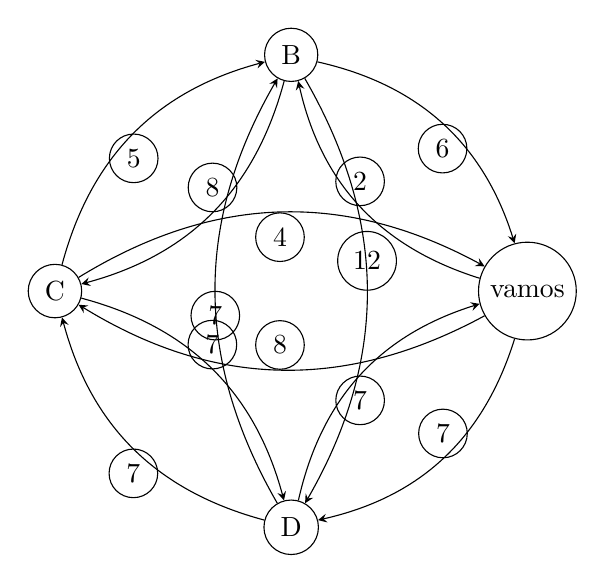
\begin{tikzpicture}[->, >=stealth, node distance=2cm, every node/.style={circle, draw}]
\node (0) at (0*360/4:3cm) {vamos};
\node (1) at (1*360/4:3cm) {B};
\node (2) at (2*360/4:3cm) {C};
\node (3) at (3*360/4:3cm) {D};
\draw (0) to[bend left] node[above] {2} (1);
\draw (1) to[bend left] node[below] {6} (0);
\draw (0) to[bend left] node[above] {8} (2);
\draw (2) to[bend left] node[below] {4} (0);
\draw (0) to[bend left] node[above] {7} (3);
\draw (3) to[bend left] node[below] {7} (0);
\draw (1) to[bend left] node[above] {8} (2);
\draw (2) to[bend left] node[below] {5} (1);
\draw (1) to[bend left] node[above] {12} (3);
\draw (3) to[bend left] node[below] {7} (1);
\draw (2) to[bend left] node[above] {7} (3);
\draw (3) to[bend left] node[below] {7} (2);
\end{tikzpicture}
\section*{Descripción}
Reporte automático del algoritmo de Floyd--Warshall. Se muestran D(0) y P(0), todas las tablas intermedias D(k) y P(k) con cambios resaltados, y el resultado final.

\begin{table}[H]\centering
\caption{D(0) -- matriz de distancias inicial}
\rowcolors{2}{white}{white}
\begin{tabular}{l r r r r}
\toprule
 & \textbf{vamos} & \textbf{B} & \textbf{C} & \textbf{D}\\\midrule
\textbf{vamos} & 0 & 2 & 8 & 7 \\
\textbf{B} & 6 & 0 & 8 & 12 \\
\textbf{C} & 4 & 5 & 0 & 7 \\
\textbf{D} & 7 & 7 & 7 & 0 \\
\bottomrule
\end{tabular}
\end{table}

\begin{table}[H]\centering
\caption{P(0) -- matriz de siguiente salto inicial}
\rowcolors{2}{white}{white}
\begin{tabular}{l c c c c}
\toprule
 & \textbf{vamos} & \textbf{B} & \textbf{C} & \textbf{D}\\\midrule
\textbf{vamos} & - & B & C & D \\
\textbf{B} & vamos & - & C & D \\
\textbf{C} & vamos & B & - & D \\
\textbf{D} & vamos & B & C & - \\
\bottomrule
\end{tabular}
\end{table}

\begin{table}[H]\centering
\caption{D(1)}
\rowcolors{2}{white}{white}
\begin{tabular}{l r r r r}
\toprule
 & \textbf{vamos} & \textbf{B} & \textbf{C} & \textbf{D}\\\midrule
\textbf{vamos} & 0 & 2 & 8 & 7 \\
\textbf{B} & 6 & 0 & 8 & 12 \\
\textbf{C} & 4 & 5 & 0 & 7 \\
\textbf{D} & 7 & 7 & 7 & 0 \\
\bottomrule
\end{tabular}
\end{table}

\begin{table}[H]\centering
\caption{P(1)}
\rowcolors{2}{white}{white}
\begin{tabular}{l c c c c}
\toprule
 & \textbf{vamos} & \textbf{B} & \textbf{C} & \textbf{D}\\\midrule
\textbf{vamos} & \cellcolor{yellow!30}vamos & B & C & D \\
\textbf{B} & vamos & \cellcolor{yellow!30}vamos & C & D \\
\textbf{C} & vamos & B & \cellcolor{yellow!30}vamos & D \\
\textbf{D} & vamos & B & C & \cellcolor{yellow!30}vamos \\
\bottomrule
\end{tabular}
\end{table}

\begin{table}[H]\centering
\caption{D(2)}
\rowcolors{2}{white}{white}
\begin{tabular}{l r r r r}
\toprule
 & \textbf{vamos} & \textbf{B} & \textbf{C} & \textbf{D}\\\midrule
\textbf{vamos} & 0 & 2 & 8 & 7 \\
\textbf{B} & 6 & 0 & 8 & 12 \\
\textbf{C} & 4 & 5 & 0 & 7 \\
\textbf{D} & 7 & 7 & 7 & 0 \\
\bottomrule
\end{tabular}
\end{table}

\begin{table}[H]\centering
\caption{P(2)}
\rowcolors{2}{white}{white}
\begin{tabular}{l c c c c}
\toprule
 & \textbf{vamos} & \textbf{B} & \textbf{C} & \textbf{D}\\\midrule
\textbf{vamos} & vamos & B & C & D \\
\textbf{B} & vamos & vamos & C & D \\
\textbf{C} & vamos & B & vamos & D \\
\textbf{D} & vamos & B & C & vamos \\
\bottomrule
\end{tabular}
\end{table}

\begin{table}[H]\centering
\caption{D(3)}
\rowcolors{2}{white}{white}
\begin{tabular}{l r r r r}
\toprule
 & \textbf{vamos} & \textbf{B} & \textbf{C} & \textbf{D}\\\midrule
\textbf{vamos} & 0 & 2 & 8 & 7 \\
\textbf{B} & 6 & 0 & 8 & 12 \\
\textbf{C} & 4 & 5 & 0 & 7 \\
\textbf{D} & 7 & 7 & 7 & 0 \\
\bottomrule
\end{tabular}
\end{table}

\begin{table}[H]\centering
\caption{P(3)}
\rowcolors{2}{white}{white}
\begin{tabular}{l c c c c}
\toprule
 & \textbf{vamos} & \textbf{B} & \textbf{C} & \textbf{D}\\\midrule
\textbf{vamos} & vamos & B & C & D \\
\textbf{B} & vamos & vamos & C & D \\
\textbf{C} & vamos & B & vamos & D \\
\textbf{D} & vamos & B & C & vamos \\
\bottomrule
\end{tabular}
\end{table}

\begin{table}[H]\centering
\caption{D(4)}
\rowcolors{2}{white}{white}
\begin{tabular}{l r r r r}
\toprule
 & \textbf{vamos} & \textbf{B} & \textbf{C} & \textbf{D}\\\midrule
\textbf{vamos} & 0 & 2 & 8 & 7 \\
\textbf{B} & 6 & 0 & 8 & 12 \\
\textbf{C} & 4 & 5 & 0 & 7 \\
\textbf{D} & 7 & 7 & 7 & 0 \\
\bottomrule
\end{tabular}
\end{table}

\begin{table}[H]\centering
\caption{P(4)}
\rowcolors{2}{white}{white}
\begin{tabular}{l c c c c}
\toprule
 & \textbf{vamos} & \textbf{B} & \textbf{C} & \textbf{D}\\\midrule
\textbf{vamos} & vamos & B & C & D \\
\textbf{B} & vamos & vamos & C & D \\
\textbf{C} & vamos & B & vamos & D \\
\textbf{D} & vamos & B & C & vamos \\
\bottomrule
\end{tabular}
\end{table}

\section*{Distancias y rutas óptimas}
\begin{table}[H]\centering
\caption{D(final)}
\rowcolors{2}{white}{white}
\begin{tabular}{l r r r r}
\toprule
 & \textbf{vamos} & \textbf{B} & \textbf{C} & \textbf{D}\\\midrule
\textbf{vamos} & 0 & 2 & 8 & 7 \\
\textbf{B} & 6 & 0 & 8 & 12 \\
\textbf{C} & 4 & 5 & 0 & 7 \\
\textbf{D} & 7 & 7 & 7 & 0 \\
\bottomrule
\end{tabular}
\end{table}

\begin{table}[H]\centering
\caption{P(final)}
\rowcolors{2}{white}{white}
\begin{tabular}{l c c c c}
\toprule
 & \textbf{vamos} & \textbf{B} & \textbf{C} & \textbf{D}\\\midrule
\textbf{vamos} & vamos & B & C & D \\
\textbf{B} & vamos & vamos & C & D \\
\textbf{C} & vamos & B & vamos & D \\
\textbf{D} & vamos & B & C & vamos \\
\bottomrule
\end{tabular}
\end{table}

\subsection*{Listado de rutas (todas las parejas i $\neq$ j)}
\begin{longtable}{llp{0.65\textwidth}}
\toprule
\textbf{Origen} & \textbf{Destino} & \textbf{Ruta óptima (con saltos)}\\\midrule
vamos & B & vamos → B (distancia = 2)\\
vamos & C & vamos → C (distancia = 8)\\
vamos & D & vamos → D (distancia = 7)\\
B & vamos & B → vamos (distancia = 6)\\
B & C & B → C (distancia = 8)\\
B & D & B → D (distancia = 12)\\
C & vamos & C → vamos (distancia = 4)\\
C & B & C → B (distancia = 5)\\
C & D & C → D (distancia = 7)\\
D & vamos & D → vamos (distancia = 7)\\
D & B & D → B (distancia = 7)\\
D & C & D → C (distancia = 7)\\
\bottomrule
\end{longtable}
\end{document}